\section{Introduction}

This lab, focusing on the concept of conservation of energy, will attempt to relate the changes in gravitational potential energy and kinetic energy in a simple system.

\section{Procedure}

A track is placed level, with the motion sensor attached at one end and a super pulley at another.
The cart is placed on the track, and a thread is attached to the cart and wound around the super pulley, allowing the other end to dangle.
The segment of the thread from the cart to the pulley is adjusted to be as horizontal as possible.

A small weight is attached to the other end of the thread, and the masses of the weight and the cart are adjusted until the cart would accelerate at a slow pace towards the pulley.

\begin{figure}[h]

\begin{center}
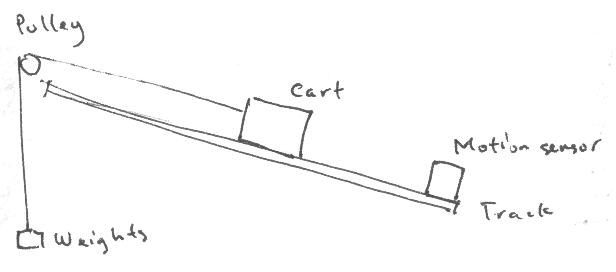
\includegraphics[scale=0.5]{content/fig1}
\end{center}

\caption{The setup of this lab.}

\end{figure}

For the first batch of tests, the track was simply released, and the velocity of the cart as it accelerated towards the pulley was recorded.

For the next batch of tests, the track was placed at an angle, with the pulley higher than the cart.
Again, the velocity of the cart was recorded.

\section{Results and Discussion}

\subsection{Questions}

\begin{enumerate}

\item What is the potential energy of the system before releasing the cart? After one second? After two?

The potential energy of the cart before the cart is released (more specifically, when the cart is at rest) we can define to be 0 Joules, in all cases.
Since it is moving downwards, the potential energy is decreasing as time goes on, since we have defined the positive direction as upwards.

Our readings are not very well defined at the one second mark, so for purposes of these questions, they will be taken at the two and three second marks.

At two seconds, the potential energies of the flat and angled tracks are roughly 0.005J and 0.237J, respectively.

At three seconds, they are 0.127J and 0.494J.

\item What is the kinetic energy of the system before releasing the cart? After one second? After two?

The kinetic energy before the cart is released is defined to be 0, since kinetic energy (K) in a system is usually defined to be \begin{math}K = \frac{1}{2}mv^2\end{math}.

Similarly, at the two second mark, the kinetic energy is roughly 0.004J and 0.23J, for the flat and angled tracks.

At the three second marks, the energies are 0.13J and 0.50J.

\item What is the velocity of the hanger as a function of its height?

All of the change in distance the hanger has gone through should, if all energy in the system is conserved, become kinetic energy.
As such, we can say that \begin{math}mgh = \frac{1}{2}mv^2\end{math}.

Solving for v, we get \begin{math}v = \sqrt{2gh}\end{math}.

\item What is the velocity of the cart as a function of hanger height?

The equation will be the same as the velocity of the hanger as a function of height, except that the resulting v will be aligned along the track, instead of vertically.

\item Is the total energy of this system conserved?

Technically, no, it shouldn't be, due to the presence of forces like friction, that may cause the energy be converted into forms that our setup was unable to account for.

If a larger system, including things such as the heat change of the devices, were used instead, then it is quite possible that the energy would appear to be conserved in the end.

In practice, the effects of friction on the system we were working with was very small to the point of possibly being negligible, giving the system the appearance of conserving all energies involved.

\item How much work is done by friction in the first second?

Starting from as many constants as possible, we can find the respective velocities and distances traveled by stating that \begin{math}m_w g = a (m_c + m_w) \end{math}, where \begin{math}m_w\end{math}
is the mass of the weights used, \begin{math}m_c\end{math} is the mass of the carts, and a is the acceleration of the system.
Thus, the theoretical acceleration involved is \begin{math}a = \frac{m_w g}{m_c + m_w}\end{math}.

From the acceleration, we can find the velocity (\begin{math}at\end{math}) and distance moved (\begin{math}\frac{1}{2}at^2\end{math}) at any time.

Thus, by applying the idea that the kinetic energy, \begin{math}\frac{1}{2}mv^2\end{math}, should be calculable, we can find the difference between our theoretical maximum and our actual measured values.
That difference should be the amount of energy removed by friction.

However, for our data, the one-second mark holds rather suspect data.
As such, the best assessment with the data we have can be done at the two second mark.
The result is approximately 0.0127J.
The energy calculated from our actual velocity measurement was around 0.005, and thus, the difference of the two is the energy lost from our friction.
As noted, it's an extremely small value, and well outside the significant figures of our measurements.

\item How much work is done by friction in the next second?

Applying the same procedure as the previous question shows that the theoretical kinetic energy at the 3-second mark should be around 0.028J.
Our measurements, calculated at a similar location, provided 0.033J.
Again, there is a discrepency, but one small enough that it may be attributable to error in the measurements themselves.

\end{enumerate}

\subsection{Error Analysis}

The greatest source of error is probably in the fact that the distance the weight dangling from the track moved down was calculated from the time and velocity measurements on the cart.
Those measurements, in turn, were extremely inaccurate very close to the sensor and at very low speeds at that time.
Thus, it was rather impractical to determine how accurate a reading within that range was, and we took our sample out of the most consistent segment of data near the middle.

In retrospect, this was not a good idea at all --- it made several calculations very complicated.
Since the "good" data started at roughly the 1.6s mark or so on the horizontal track measurements, it meant that it was impractical to determine, exactly, what the energy of the system was at those points.

\section{Conclusion}

In theory, the kinetic energy of the cart should be somehow proportional to the gravitational potential energy change of the weight on the other end of the track.
In practice, it was fairly close, but there was some energy lost from the system due to friction.
Presumably, that energy became heat, but as we had no means to measure that effectively, we can only assume that the energy lost is directly proportional to the frictional force of the system.

